\documentclass{article}
\usepackage{tpack}

\title{ES572 - Circuitos Lógicos}
\author{Guilherme Nunes Trofino}
\authorRA{217276}
\project{Resumo Teórico}


\begin{document}
    \maketitle
\newpage

    \tableofcontents
\newpage

    \section{Introdução}
        \paragraph{Apresentação}Neste documento será descrito as informações necessárias para compreensão e solução de exercícios relacionados a disciplina \thetitle. Note que este documento são notas realizadas por \theauthor , em \today.

\begin{multicols}{2}
    \raggedcolumns

    \subsection{Informação}
        \paragraph{Definição}Informação são dados comunicados ou recebidos que resolvem incertezas sobre um fato ou circunstância específica. Assim, dada uma variável aleatória discreta $x$ com as seguintes condições:
            \begin{enumerate}[noitemsep]
                \item Possíveis Valores: $x \in \{x_{1},...,x_{n}\}$;
                \item Probabilidades Associadas: $\{p_{1},...,p_{n}\}$;
            \end{enumerate}
        Desta forma, considera-se $I(x_{i})$ que a \textbf{Quantidade de Informação Recebida}, medida em \texttt{bits}, será relacionada por:
            \begin{equation}
                \boxed{
                    I(x_{i}) = \log_{2}\left(\frac{1}{p_{i}}\right)
                }
            \end{equation}
        Nota-se trata-se de uma informação relacionada apenas ao evento analisado. Além disso, eventos de baixa probabilidade transportam mais informação.

    \columnbreak

    \subsection{Entropia}
        \paragraph{Definição}Dada uma variável aleatória $x$ então sua \textbf{Entropia} $H(x)$ será a quantidade média de informação recebida ao conhecer seu valor, sendo descrita pela equação abaixo:
            \begin{equation*}
                H(x) = E(I(x)) = \sum_{i=1}^{N}p_{i}\log_{2}\left(\frac{1}{p_{i}}\right)
            \end{equation*}
        Onde $E(x)$ representa a \textbf{Esperança} da variável $x$, podendo ser simplificada para:
            \begin{equation}
                \boxed{
                    H(x) = -\sum_{i=1}^{N}p_{i}\log_{2}p_{i}
                }
            \end{equation}
        Nota-se que trata-se de uma informação relacionada apenas ao processo analisado:
            \begin{enumerate}[noitemsep]
                \item Quanto mais baixa, mais previsível; 
                \item Quanto mais alta, mais imprevisível; 
            \end{enumerate}
\end{multicols}
        
        \subsection{Codificação}
            \paragraph{Definição}Mapeamento \textbf{biunívoco}, cada elemento associado a um único contraelemento, entre cadeias de bits e os membros do conjunto de dados a serem condificados. Classificados em:
                \begin{enumerate}[rightmargin = \leftmargin]
                    \item \textbf{Comprimento Fixo:} Caso todos os símbolos ocorram com a mesma probabilidade, geralmente utiliza-se este método;
                        \begin{enumerate}[noitemsep, rightmargin = \leftmargin]
                            \item \texttt{Vantagens:}
                                \begin{enumerate}[noitemsep, rightmargin = \leftmargin]
                                    \item Todas as folhas possuem a mesma distância da raiz;
                                    \item Acesso Aleatório: Variáveis podem ser lidas em qualquer trecho da codificação;
                                \end{enumerate}

                            \item \texttt{Entropia:} Considera-se uma variável aleatória X que assume valores entre $N$ possibilidades equiprováveis será:
                                \begin{equation}
                                    \boxed{
                                        H(x) = \sum_{i=1}^{N}p_{i}\log_{2}\left(\frac{1}{p_{i}}\right) = \sum_{i=1}^{N}\frac{1}{N}\log_{2}(N)
                                    }
                                \end{equation}
                            Desta forma, uma codificação \textbf{ótima} terá $N = 2^{k}$, onde $k \in \mathbb{N}$.
                        \end{enumerate}

                    \item \textbf{Comprimento Variável:} Caso todos os símbolos não ocorram com a mesma probabilidade, geralmente utiliza-se este método;
                        \begin{enumerate}[noitemsep, rightmargin = \leftmargin]
                            \item \texttt{Vantagens:}
                                \begin{enumerate}[noitemsep, rightmargin = \leftmargin]
                                    \item Flexibilidade para se aproximar da codificação \textbf{ideal};
                                    \item Necessária para compresão de arquivos, como descrito por \textbf{Huffman};
                                \end{enumerate}

                            \item \texttt{Entropia:} Considera-se uma variável aleatória X que assume valores entre $N$ possibilidades equiprováveis será:
                                \begin{equation}
                                    \boxed{
                                        H(x) = \sum_{i=1}^{N}p_{i}\log_{2}\left(\frac{1}{p_{i}}\right)
                                    }
                                \end{equation}
                            Desta forma, uma codificação \textbf{ótima} terá:
                                \begin{enumerate}[noitemsep, rightmargin = \leftmargin]
                                    \item \texttt{Codificação Curta:} Se $x_{i}$ tiver uma probabilidade alta;
                                    \item \texttt{Codificação Longa:} Se $x_{i}$ tiver uma probabilidade baixa;
                                \end{enumerate}
                        \end{enumerate}

                    \item \textbf{Codificação Ambígua:} Organização não única dos caracteres envolvidos o que pode gerar problemas de interpretação dos dados. Deve ser \textbf{evitada};

                \end{enumerate}
            Será necessário evitar codificações ambíguas, pois poderá haver incerteza de informação neste caso. Desta forma, uma árvore binária deve ser criada para validar se a codificação é válida, alocando as variáveis nos terminais das ramificações.

        \subsection{Algoritmo de Huffman}
            \paragraph{Definição}Algoritmo para construção de uma \textbf{Árvore Binária Ótima}, isto é uma codificação que possua entropia próxima a mínima necessária. Aplica-se os seguintes passos:
                \begin{enumerate}[rightmargin = \leftmargin]
                    \item Criação de uma sub-árvore com os símbolos de \textbf{menor} probabilidade, associando-a o somatório de suas possibilidades;
                    \item Seleção de dois símbolos ou sub-árvores com menores probabilidades e as combine em uma nova sub-árvore;
                    \begin{enumerate}[noitemsep, rightmargin = \leftmargin]
                        \item Caso hajam símbolos ou sub-árvores com mesma probabilidade, escolha arbitrariamente;
                    \end{enumerate}
                \end{enumerate}
            Consequência deste algoritmo:
                \begin{itemize}[rightmargin = \leftmargin]
                    \item Todas as codificações apresentam o mesmo comprimento esperado, logo a mesma eficiência, independente dos rótulos empregados para cada ramificação;
                    \item Desempenhos mais próximos da entropia podem ser obtidos com sequências maiores, normalmente aplicadas em algoritmos de compressão como \texttt{LZW};
                \end{itemize}

    \begin{multicols}{2}
        \begin{figure}[H]
            \centering
            \begin{forest} % from https://tex.stackexchange.com/a/304002/121799
                for tree={
                    s sep = 10mm,   % Horizontal Distance
                    l = 0mm,        % Vertical Distance
                    where n children={0}{ev}{iv},
                    l+=8mm,
                    if n=1{
                        edge label={
                            node [midway, left] {0}
                        }
                    }{
                        edge label={
                            node [midway, right] {1}
                        }
                    }
                }
                [100
                    [60
                        [A] [B]
                    ]
                    [40
                        [C]
                        [20
                            [D] [E]
                        ]
                    ]
                ]
            \end{forest}
            \caption{Representação da Árvore de Huffman}
        \end{figure} \noindent

        \columnbreak\noindent
        Considera-se como exemplo a seguinte distribuição de probabilidades:
            \begin{table}[H]
                \centering
                \begin{tabular}[]{ccc}\hline
                    Símbolos & Probabilidade & Codificação\\\hline
                    A & 30 & 00\\
                    B & 30 & 01\\
                    C & 20 & 10\\
                    D & 10 & 110\\
                    E & 10 & 111\\\hline
                \end{tabular}
                \caption{Probabilidades dos Símbolos}\label{table:Huffman}
            \end{table}
    \end{multicols}

        \subsection{Distância de Hamming}
            \paragraph{Definição}Representa o número de posições nos quais os dígitos correspondentes \textbf{diferem} entre si, como representado abaixo:
                \begin{table}[H]
                    \centering
                    \begin{tabular}[]{cc}\hline
                        Original  & Palavra Código\\\hline
                        0110 0100 & 01\textcolor{red}{0}0 \textcolor{red}{1}100\\\hline
                    \end{tabular}
                    \caption{Representação da Distância de Hamming}\label{table:HammingDefinition}
                \end{table}\noindent

        \subsubsection{Deteção de \texttt{Erro de 1 bit}}
            \paragraph{Definição}Criação de palavras código válidas, de modo que um erro de um \textbf{único} \texttt{bit} não produza outra palavra de código válida. Desta forma, será necessário uma codificação cuja distância de Hamming entre quaisquer palavras válidas seja de \textbf{pelo menos} 2.

            \paragraph{Aplicação}Adiciona-se um \texttt{bit} em qualquer palavra válida para que o número total de \texttt{bits 1} seja:
                \begin{enumerate}[noitemsep, rightmargin = \leftmargin]
                    \item \textbf{Paridade Par:} Possui um número par de \texttt{bits 1}. Representado com \texttt{bit 0};
                    \item \textbf{Paridade Ímpar:} Possui um número ímpar de \texttt{bits 1}. Representado com \texttt{bit 1};
                \end{enumerate}

            \paragraph{Generalização}Considere um símbolo codificado qualquer, para \textbf{Detectar} um número $E$ de erros será necessário uma distância mínima de Hamming $E+1$ entre as palavras de código. Além disso, a \textbf{Correção} um número $E$ de erros será necessário uma distância mínima de Hamming $2E+1$.

        \subsubsection{Codificação de Hamming \texttt{(15, 11)}}
            \paragraph{Definição}Organização de dados em \texttt{15 bits}, \texttt{11 bits} de dados e \texttt{4 bits} são redundância. Desta forma, os \texttt{bits} redundantes são suficientes para determinar a posição de qualquer erro de \texttt{1 bit} presente nos dados.

            \paragraph{Aplicação}Organize os \texttt{11 bits} de dados sequencialmente nos espaços brancos de uma matriz 4x4 como representado abaixo:
                \begin{table}[H]
                    \centering\begin{tabular}{|c|c|c|c|}\hline
                        \cellcolor{blue!40}\mycell{x}{0} & \cellcolor{red!40}\mycell{p}{1} & \cellcolor{red!40}\mycell{p}{2}  & \mycell{1}{3}\\\hline
                        \cellcolor{red!40}\mycell{p}{4}  & \mycell{0}{5}                   & \mycell{1}{6}                    & \mycell{0}{7}\\\hline
                        \cellcolor{red!40}\mycell{p}{8}  & \mycell{0}{9}                   & \mycell{1}{10}                   & \mycell{0}{11}\\\hline
                        \mycell{1}{12}                   & \mycell{0}{13}                  & \mycell{0}{14}                   & \mycell{1}{15}\\\hline
                    \end{tabular}
                    \caption{Codificação de Hamming}
                    \label{table:HammingCode}
                \end{table}\noindent
            Na sequência preenche-se os \textcolor{red!80}{\texttt{bits de paridade}}, apresentados nas posições com \textcolor{red!80}{p}, representando a paridade de cada \textbf{subgrupo} possuam como representado abaixo:
                \begin{table}[H]
                    \centering
                    \begin{tabular}{|c|c|c|c|}\hline
                        \mycell{x}{0}  & \cellcolor{red!40}\mycell{0}{1}   & \mycell{p}{2}  & \cellcolor{gray!50}\mycell{1}{3}\\\hline
                        \mycell{p}{4}  & \cellcolor{gray!50}\mycell{0}{5}  & \mycell{1}{6}  & \cellcolor{gray!50}\mycell{0}{7}\\\hline
                        \mycell{p}{8}  & \cellcolor{gray!50}\mycell{0}{9}  & \mycell{1}{10} & \cellcolor{gray!50}\mycell{0}{11}\\\hline
                        \mycell{1}{12} & \cellcolor{gray!50}\mycell{0}{13} & \mycell{0}{14} & \cellcolor{gray!50}\mycell{1}{15}\\\hline
                    \end{tabular}
                    \quad
                    \begin{tabular}{|c|c|c|c|}\hline
                        \mycell{x}{0}  & \mycell{0}{1}  & \cellcolor{red!40}\mycell{0}{2}   & \cellcolor{gray!50}\mycell{1}{3}\\\hline
                        \mycell{p}{4}  & \mycell{0}{5}  & \cellcolor{gray!50}\mycell{1}{6}  & \cellcolor{gray!50}\mycell{0}{7}\\\hline
                        \mycell{p}{8}  & \mycell{0}{9}  & \cellcolor{gray!50}\mycell{1}{10} & \cellcolor{gray!50}\mycell{0}{11}\\\hline
                        \mycell{1}{12} & \mycell{0}{13} & \cellcolor{gray!50}\mycell{0}{14} & \cellcolor{gray!50}\mycell{1}{15}\\\hline
                    \end{tabular}
                    \quad
                    \begin{tabular}{|c|c|c|c|}\hline
                        \mycell{x}{0}                     & \mycell{0}{1}                     & \mycell{0}{2}                     & \mycell{1}{3}\\\hline
                        \cellcolor{red!40}\mycell{1}{4}   & \cellcolor{gray!50}\mycell{0}{5}  & \cellcolor{gray!50}\mycell{1}{6}  & \cellcolor{gray!50}\mycell{0}{7}\\\hline
                        \mycell{p}{8}                     & \mycell{0}{9}                     & \mycell{1}{10}                    & \mycell{0}{11}\\\hline
                        \cellcolor{gray!50}\mycell{1}{12} & \cellcolor{gray!50}\mycell{0}{13} & \cellcolor{gray!50}\mycell{0}{14} & \cellcolor{gray!50}\mycell{1}{15}\\\hline
                    \end{tabular}
                    \quad
                    \begin{tabular}{|c|c|c|c|}\hline
                        \mycell{x}{0}                     & \mycell{0}{1}                     & \mycell{0}{2}                     & \mycell{1}{3}\\\hline
                        \mycell{1}{4}                     & \mycell{0}{5}                     & \mycell{1}{6}                     & \mycell{0}{7}\\\hline
                        \cellcolor{red!40}\mycell{1}{8}   & \cellcolor{gray!50}\mycell{0}{9}  & \cellcolor{gray!50}\mycell{1}{10} & \cellcolor{gray!50}\mycell{0}{11}\\\hline
                        \cellcolor{gray!50}\mycell{1}{12} & \cellcolor{gray!50}\mycell{0}{13} & \cellcolor{gray!50}\mycell{0}{14} & \cellcolor{gray!50}\mycell{1}{15}\\\hline
                    \end{tabular}
                    \caption{Grupos de Hamming}
                    \label{table:HammingGroups}
                \end{table}\noindent
            Neste ponto pode-se detectar e localizar \texttt{erros de 1 bit}. Na sequência preenche-se o \textcolor{blue!80}{\texttt{bit de paridade do conjunto}} para paridade do \textbf{grupo} como representado abaixo:
                \begin{table}[H]
                    \centering
                    \begin{tabular}{|c|c|c|c|}\hline
                        \cellcolor{blue!40}\mycell{1}{0} & \mycell{0}{1}  & \mycell{0}{2}  & \mycell{1}{3}\\\hline
                        \mycell{1}{4}                    & \mycell{0}{5}  & \mycell{1}{6}  & \mycell{0}{7}\\\hline
                        \mycell{1}{8}                    & \mycell{0}{9}  & \mycell{1}{10} & \mycell{0}{11}\\\hline
                        \mycell{1}{12}                   & \mycell{0}{13} & \mycell{0}{14} & \mycell{1}{15}\\\hline
                    \end{tabular}
                    \caption{Codificação Hamming Estendida}
                    \label{table:HammingFinal}
                \end{table}\noindent
            Neste ponto pode-se localizar \texttt{erros de 2 bits}.

        \subsubsection{Decodificação de Hamming \texttt{(15, 11)}}
            \paragraph{Definição}Interpretação dos dados recebidos na \textbf{Configuração de Hamming}, analisando os \texttt{15, ou 16, bits} codificados como descrito abaixo:
                \begin{enumerate}[rightmargin = \leftmargin]
                    \item \textbf{Transmissão Correta:} 
                        \begin{enumerate}[noitemsep, rightmargin = \leftmargin]
                            \item Não houve erro nos \textcolor{red!80}{\texttt{bits de paridade}};
                            \item Não houve erro no \textcolor{blue!80}{\texttt{bit de paridade do conjunto}};
                        \end{enumerate}

                    \item \textbf{Transmissão com} \texttt{Erro de 1 bit}:
                        \begin{enumerate}[noitemsep, rightmargin = \leftmargin]
                            \item Houve erro em pelo menos um dos \textcolor{red!80}{\texttt{bits de paridade}};
                            \item Houve erro no \textcolor{blue!80}{\texttt{bit de paridade do conjunto}};
                        \end{enumerate}

                    \item \textbf{Transmissão com} \texttt{Erro de 2 bit}:
                        \begin{enumerate}[noitemsep, rightmargin = \leftmargin]
                            \item Houve erro em pelo menos um dos \textcolor{red!80}{\texttt{bits de paridade}};
                            \item Não houve erro no \textcolor{blue!80}{\texttt{bit de paridade do conjunto}};
                        \end{enumerate}
                \end{enumerate}

    \section{Abstração Digital}
        \paragraph{Apresentação}Depois de discutido como codificar informações como sequência de bits será necessário elaborar uma forma para codifica-la fisicamente que atenda aos seguintes características:
            \begin{enumerate}[noitemsep]
                \item \textbf{Pequeno:} Necessite de pouco espaço para armazenamento;
                \item \textbf{Barato:} Economicamente acessível para produção;
                \item \textbf{Estável:} Não apresentará mudanças durante seu uso;
                \item \textbf{Veloz:} Fácil de acessar, transformar, combinar, transmitir e armazenar;
            \end{enumerate}
        No mundo, não quântico, não é digital e são afetados por imperfeições que devem ser consideradas na descrição de modelo de conversão que consigo manter a precisão necessária para aplicação desejada.

        \subsection{Processamento Digital}
            \paragraph{Definição}Conversão, manipulação e utilização de sinais digitais para interpretação de fenômenos físicos estudados. Isso demandará algumas definições de conceitos descritas na sequência.

            \subsubsection{Conversão Digital}
                \paragraph{Definição}Inicialmente será necessário determinar como os sinais analógicos, medições reais, serão convertido para sinais digitais para que então possam ser trabalhados, buscando métodos que atendam as condições de codificações como a representada a seguir:
                    \begin{equation}
                        \boxed{
                            V = 
                            \begin{cases}
                                0,                      & \text{se } V \leq V_{OL}\\
                                \text{margem de erro},  & \text{se } V_{OL} \leq V \leq V_{IL}\\
                                \text{zona proíbida},   & \text{se } V_{IL} \leq V \leq V_{IH}\\
                                \text{margem de erro},  & \text{se } V_{IH} \leq V \leq V_{OH}\\
                                1,                      & \text{se } V \geq V_{OH}\\
                            \end{cases}
                        }
                    \end{equation}
                Onde:
                    \begin{enumerate}[noitemsep]
                        \item \texttt{Nível Lógico 0:} Caso $V$ seja menor ou igual ao \textbf{Threshold Low} $V_{OL}$;

                        \item \texttt{Nível Lógico 1:} Caso $V$ seja maior ou igual ao \textbf{Threshold High} $V_{OH}$;
                    \end{enumerate}
                Note que desta forma o sinal estará protegido de pequenos ruídos pois não poderá passar de um nível lógico para o outro diretamente.

        \subsubsection{Atraso de Propagação, $t_{PD}$}
            \paragraph{Definição}Limitante superior para o atraso de entradas válidas para saídas válidas causado pela presença intrínseca de capacitâncias e resistências na construção dos dispositivos como representado pelo seguinte gráfico:

        \subsubsection{Atraso de Contaminação, $t_{CD}$}
            \paragraph{Definição}Limitante inferior para o atraso de entradas inválidas para saídas inválidas causado pela presença intrínseca de ruídos ou interferência na atuação dos dispositivos como representado pelo seguinte gráfico:

        \subsection{Dispositivos Combinacionais}
            \paragraph{Definição}Componente eletrônico que atende as seguintes especificações:
                \begin{enumerate}[rightmargin = \leftmargin]
                    \item \textbf{Comunicação:} Necessidades para interface com o dispositivo apresentando:
                        \begin{enumerate}[noitemsep]
                            \item \texttt{Entradas:} Ao menos uma entrada digital;
                            \item \texttt{Saídas:} Ao menos uma saída digital;
                        \end{enumerate}

                    \item \textbf{Especificação Funcional:} Qualquer saída será obtida por uma combinação possível das entradas válidas;

                    \item \textbf{Especificação Temporal:} Há um \texttt{Tempo de Propagação} $t_{PD}$ mínimo necessário para que o dispositivo calcule a saída a partir de suas entradas válidas;
                \end{enumerate}
            Além disso, um conjunto de elementos interconectados será combinacional se não viola nenhuma das seguintes regras:
                \begin{enumerate}[noitemsep]
                    \item \textbf{Condição 1:} Cada elemento individual é combinacional;

                    \item \textbf{Condição 2:} Cada entrada é conectada a uma, e apenas uma, saída ou fornecimento externo;

                    \item \textbf{Condição 3:} Não há ciclos diretos;
                \end{enumerate}

        \subsubsection{Buffer}
            \paragraph{Definição}Dispositivo eletrônico que transfere tensão, mantendo sua estabilidade apesar de logicamente não alterá-lo visto que ao longo da transmisssão o acumulo de ruídos poderia modificar o sinal transmitido.

            \paragraph{Representação}Dispositivo apresentará a seguinte tabela verdade e representação em circuitos:
                \begin{multicols}{2}
                    \begin{table}[H]
                        \centering  
                        \begin{tabular}[]{c|c}\hline
                            in & out\\\hline
                            0  & 0\\
                            1  & 1\\\hline
                        \end{tabular}
                        \caption{Tabela Verdade Buffer}
                    \end{table}
                    \columnbreak\noindent
                    \begin{figure}[H]
                        \centering
                        \begin{circuitikz}
                            \ctikzset{component text=left}
                            \draw
                            (0,0) node[buffer] (myPort) {}
                            (myPort.in)  node [anchor = east] {in}
                            (myPort.out) node [anchor = west] {out};
                        \end{circuitikz} 
                        \caption{Representação Buffer}
                    \end{figure} \noindent
                \end{multicols}\noindent
            Além disso, a representação da \textbf{Curva Característica de Transferências}, relação entre a tensão de entrada com a tensão de saída, será dada pelo seguinte gráfico:
                [todo add gráfico]

        \subsection{CMOS}
            \paragraph{Definição}Metodologia de projeto de circuitos digitais dominante no mercado por seu baixo consumo de energia que deve atender aos seguintes requisitos:
                \begin{enumerate}[noitemsep, rightmargin = \leftmargin]
                    \item \textbf{Pull-Down:} Conexão com baixa tensão através de NMOS;
                    \item \textbf{Pull-Up:} Conexão com alta tensão através de PMOS;
                    \item \textbf{Circuitos Duais:} ;
                \end{enumerate}

            \subsubsection{Inversor}
                \paragraph{Definição}Dispositivo eletrônico que inverte sua tensão entrada, valores de entrada alto implicam saída baixa e valores baixos de entrada implicam saída alta.

                \paragraph{Representação}Dispositivo apresentará a seguinte tabela verdade e representação em circuitos:
                    \begin{multicols}{2}
                        \begin{table}[H]
                            \centering  
                            \begin{tabular}[]{c|c}\hline
                                in & out\\\hline
                                0  & 1\\
                                1  & 0\\\hline
                            \end{tabular}
                            \caption{Tabela Verdade Inversor}
                        \end{table}
                        \columnbreak\noindent
                        \begin{figure}[H]
                            \centering
                            \begin{circuitikz}
                                \ctikzset{component text=left}
                                \draw
                                (0, 1) node[pmos] (myPFET) {}
                                (0,-1) node[nmos] (myNFET) {}
                
                                (myPFET.G) -- (myNFET.G)
                                (myPFET.D) -- (myNFET.D)
                
                                (-1.48,0) to[short, o-*] (-0.98,0)
                                ( 0,0) to[short, *-o] ( 0.5, 0)
                
                                (-1.48,0) node[left]{$v_{i}$}
                                ( 0.5,0) node[right]{$v_{o}$}
                
                                (myPFET.S) node[vcc]{$v_{\text{DD}}$}
                                (myNFET.S) node[tlground]{$v_{\text{SS}}$};
                            \end{circuitikz} 
                            \caption{Representação Inversor}
                        \end{figure} \noindent
                    \end{multicols}\noindent
                Além disso, a representação da \textbf{Curva Característica de Transferências}, relação entre a tensão de entrada com a tensão de saída, será dada pelo seguinte gráfico:
                    [todo add gráfico]
                    \begin{figure}[H]
                        \centering
                        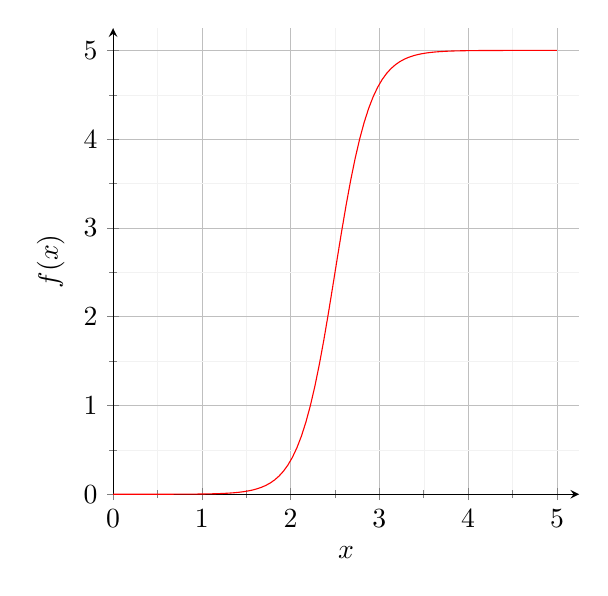
\begin{tikzpicture}
                            \begin{axis}[
                                xmin = 0, xmax = 5.25,
                                ymin = 0, ymax = 5.25,
                                width  = 7.5cm, xlabel = \(x\),
                                height = 7.5cm, ylabel = {\(f(x)\)},
                                grid = both,
                                grid style       = {line width=.1pt, draw=gray!10},
                                major grid style = {line width=.2pt, draw=gray!50},
                                minor tick num=1,
                                axis lines = left,
                            ]
                            \addplot [
                                    domain=0:5, 
                                    samples=100, 
                                    color=red,
                            ] {5/(1+exp(-5*x+12.5))};
                            % \addlegendentry{$\frac{5}{1 + e^{-5x+12.5}}$}
                            \end{axis}
                        \end{tikzpicture}
                    \end{figure}\noindent
                    \begin{figure}[H]
                        \centering
                        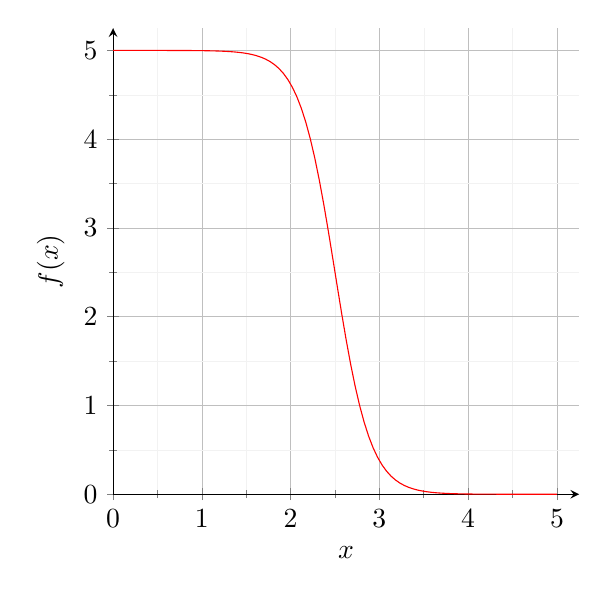
\begin{tikzpicture}
                            \begin{axis}[
                                xmin = 0, xmax = 5.25,
                                ymin = 0, ymax = 5.25,
                                width  = 7.5cm, xlabel = \(x\),
                                height = 7.5cm, ylabel = {\(f(x)\)},
                                grid = both,
                                grid style       = {line width=.1pt, draw=gray!10},
                                major grid style = {line width=.2pt, draw=gray!50},
                                minor tick num=1,
                                axis lines = left,
                            ]
                            \addplot [
                                    domain=0:5, 
                                    samples=100, 
                                    color=red,
                            ] {5/(1+exp(+5*x-12.5))};
                            % \addlegendentry{$\frac{5}{1 + e^{-5x+12.5}}$}
                            \end{axis}
                        \end{tikzpicture}
                    \end{figure}\noindent

            tempos de ligar e desligar do circuito
            circuitos lenientes
\end{document}